\documentclass[a4paper, 11pt]{article}

\usepackage{amsmath}
\usepackage{amssymb}
\usepackage{titlesec}
\usepackage[utf8]{inputenc}
\usepackage[margin=1.5cm]{geometry}
\usepackage{prftree}
\usepackage{changepage}
\usepackage{enumitem}
\usepackage{minted}
\usepackage{lmodern}
\usepackage{graphicx}
\usepackage{wrapfig}
\usepackage{ulem}
\usepackage{marvosym}
\usepackage{xcolor}
\usepackage{mathtools}
\usepackage{todonotes}
\usepackage{bm}

\title{\vspace{-2cm}Hoare Logic and Model Checking\vspace{-2cm}}
\author{}
\date{}

\setlength{\parindent}{0cm}
\setlength{\parskip}{2mm}
\setlist{nosep}

% Make ~ look more normal
\let\oldsim\sim
\renewcommand{\sim}{{\oldsim}}

\newmintinline[monospace]{text}{escapeinside=\#\#, mathescape, fontsize=\normalsize}
\newminted[monospacefigure]{text}{frame=lines, framesep=1mm, autogobble, escapeinside=\#\#, mathescape, breaklines}

\titlespacing{\section}{0mm}{2mm}{2mm}
\titlespacing{\subsection}{0mm}{2mm}{2mm}
\titlespacing{\subsubsection}{0mm}{2mm}{2mm}

\newcommand{\triple}[3]{\{#1\}\;#2\;\{#3\}}
\newcommand{\triplem}[3]{\(\triple{#1}{#2}{#3}\)}
\newcommand{\ttriple}[3]{[#1]\;#2\;[#3]}

\newcommand{\interp}[2][]{\mathcal{#1}[\![#2]\!]}

\newcommand{\lightning}{\text{\Lightning}}

\newcommand{\doubleplus}{+\kern-1.3ex+\kern0.8ex}
\newcommand{\ditto}{\text{---}\cdot\cdot\,\text{---}}

\begin{document}
\maketitle
\section*{\texttt{while} Language}
{
    \begin{minipage}[t]{0.4\textwidth}
    \vspace{-7mm}
    \begin{alignat*}{2}
    C ::=& \; &\;&\text{skip} \\
         & | &&C_1 ; C_2 \\
         & | &&X := E \\
         & | &&\text{if }B\text{ then }C_1\text{ else }C_2 \\
         & | &&\text{while }B\text{ do }C
    \end{alignat*}
    \end{minipage}
    \begin{minipage}[t]{0.5\textwidth}
    \(E\) are arithmetic expressions, can't contain program statements and don't have side effects. \(B\) are boolean expressions.
    \end{minipage}

    \subsection*{Dynamic Semantics of \texttt{while}}
    {
        Stacks are \textbf{total} functions from program variables to integers (\(s \in \text{Stack} = \text{Var} \rightarrow \mathbb{Z}\)) defining the value of every program variable.

        Define \(\interp[E]{E}(s)\) and \(\interp[B]{B}(s)\) as evaluating the expression in a stack:

        \begin{minipage}[t]{0.48\textwidth}
        \begin{align*}
        \interp[E]{N}(s) &= N \\
        \interp[E]{X}(s) &= s(X) \\
        \interp[E]{E_1 + E_2}(s) &= \interp[E]{E_1}(s) + \interp[E]{E_2}(s) \\
        ...
        \end{align*}
        \end{minipage}
        \begin{minipage}[t]{0.48\textwidth}
        \begin{align*}
        \interp[B]{\texttt{T}}(s) &= \top \\
        \interp[B]{\texttt{F}}(s) &= \bot \\
        \interp[B]{E_1 \leq E_2}(s) &= \begin{cases}
            \top & \text{, if }\interp[E]{E_1}(s) \leq \interp[E]{E_2}(s) \\
            \bot & \text{, otherwise}
        \end{cases} \\
        ...
        \end{align*}
        \end{minipage}

        \begin{gather*}
        \prftree[r]{}
        {\interp[E]{E}(s) = N}
        {\langle X:=E , s \rangle \rightarrow \langle \texttt{skip} , s[X \mapsto N] \rangle}
        \\
        \\
        \prftree[r]{}
        {\interp[B]{B}(s) = \top}
        {\langle \texttt{if }B\texttt{ then }C_1\texttt{ else }C_2, s \rangle \rightarrow \langle C_1 , s \rangle}
        \qquad
        \prftree[r]{}
        {\interp[B]{B}(s) = \bot}
        {\langle \texttt{if }B\texttt{ then }C_1\texttt{ else }C_2, s \rangle \rightarrow \langle C_2 , s \rangle}
        \\
        ...
        \end{gather*}

        A configuration can terminate: \(\exists s'.\; \langle C,s \rangle \rightarrow^* \langle \texttt{skip},s' \rangle\).

        A configuration can fail to terminate: \(\langle C,s \rangle \rightarrow^\omega\).
    }
    \subsection*{Interpretations}
    {
        Define interpretations of assertions on a specific stack.
        
        \begin{itemize}
        \item \textbf{\(\interp{P}\) is the set of stacks \(s\) which satisfy \(P\)}.
        \item \textbf{\(\interp{t}(s)\) is the value of interpreting term \(t\) in the stack \(s\)}.
        \end{itemize} 
        \vspace{-5mm}
        \begin{minipage}[t]{0.51\textwidth}
        \begin{align*}
        \interp{\bot} &= \emptyset \\
        \interp{\top} &= \text{Stack} \\
        \interp{P \vee Q} &= \interp{P} \cup \interp{Q} \\
        \interp{P \wedge Q} &= \interp{P} \cap \interp{Q} \\
        \interp{t_1 = t_2} &= \{s\in\text{Stack} \mid \interp{t_1}(s) = \interp{t_2}(s)\} \\
        \interp{p(t_1, ..., t_n)} &= \{ s\in\text{Stack} \mid \interp{p}(\interp{t_1}(s), ..., \interp{t_n}(s)) \} \\
        \interp{\forall x.\;P} &= \{s\in\text{Stack} \mid \forall N.\; s[x \mapsto N] \in \interp{P}\} \\
        \interp{\exists x.\;P} &= \{s\in\text{Stack} \mid \exists N.\; s[x \mapsto N] \in \interp{P}\}
        \end{align*}
        \end{minipage}
        \begin{minipage}[t]{0.47\textwidth}
        \begin{align*}
        \interp{B} & = \{s\in\text{Stack} \mid \interp[B]{B}(s) = \top \} \\
        \interp{f(t_1, ..., t_n)}(s) &= \interp{f}(\interp{t_1}(s), ..., \interp{t_n}(s))
        \end{align*}
        \end{minipage}

        Can now define:
        \[\vDash \triple{P}{C}{Q} \stackrel{\text{def}}{=} \forall s,s'.\; (s\in\interp{P}) \wedge (\langle C,s \rangle \rightarrow^* \langle \texttt{skip},s' \rangle) \implies s' \in \interp{Q]}\]
    }
}
\section*{\texttt{while}\(_p\) Language}
{
    \texttt{while} with pointers. Introduce new commands:
    \begin{alignat*}{2}
    C ::=& \; &\;&X := [E] \\
         & | && [E_1] := E_2 \\
         & | && X := \texttt{alloc}(E_0,...,E_n) \\
         & | && \texttt{dispose}(E)
    \end{alignat*}

    Commands are now evaluated with a heap and a stack: \(h\in\text{Heap} = (\text{Loc} \setminus \{\texttt{null}\}) \rightarrow \mathbb{Z}\), \(l\in\text{Loc} = \mathbb{N}\). The existing commands can be easily extended to handle the extra state.

    The new commands \textbf{fail} (\(\lightning\)) if the given locations aren't allocated, but otherwise have straightforward dynamic semantics. Allocating memory needs to find a contiguous block of unallocated memory to place the values in.

    \begin{gather*}
    \prftree[r]{}
    {\interp[E]{E}(s) = l}
    {l \in \text{dom}(h)}
    {h(l) = N}
    {\langle X:=[E], s, h \rangle \rightarrow \langle \texttt{skip}, s[X\mapsto N], h \rangle}
    \qquad
    \prftree[r]{}
    {\interp[E]{E}(s) = l}
    {l \notin \text{Loc}}
    {\langle X:=[E], s, h \rangle \rightarrow \lightning}
    \qquad
    \prftree[r]{}
    {\interp[E]{E}(s) = l}
    {l \notin \text{dom}(h)}
    {\langle X:=[E], s, h \rangle \rightarrow \lightning}
    \\
    \\
    \prftree[r]{}
    {\interp[E]{E_1}(s) = l}
    {l \in \text{dom}(h)}
    {\interp[E]{E_2} = N}
    {\langle [E_1]:=E_2, s, h \rangle \rightarrow \langle \texttt{skip}, s, h[l \mapsto N] \rangle}
    \qquad
    \prftree[r]{}
    {\interp[E]{E_1}(s) = l}
    {l\notin\text{Loc}}
    {\langle [E_1]:=E_2, s, h \rangle \rightarrow \lightning}
    \qquad
    \prftree[r]{}
    {\interp[E]{E_1}(s) = l}
    {l \notin \text{dom}(h)}
    {\langle [E_1]:=E_2, s, h \rangle \rightarrow \lightning}
    \\
    \\
    \prftree[r]{}
    {\interp[E]{E}(s) = l}
    {l \in \text{dom}(h)}
    {h(l) = N}
    {\langle \texttt{dispose}(E), s, h \rangle \rightarrow \langle \texttt{skip}, s, h\setminus\{(l, N)\} \rangle}
    \quad
    \prftree[r]{}
    {\interp[E]{E}(s) = l}
    {l\notin\text{Loc}}
    {\langle \texttt{dispose}(E), s, h \rangle \rightarrow \lightning}
    \quad
    \prftree[r]{}
    {\interp[E]{E}(s) = l}
    {l \notin \text{dom}(h)}
    {\langle \texttt{dispose}(E), s, h \rangle \rightarrow \lightning}
    \\
    \\
    \prftree[r]{}
    {\interp[E]{E_0}(s) = N_0}
    {...}
    {\interp[E]{E_n}(s) = N_n}
    {\forall i \in {0,...,n}.\;l+i \notin \text{dom}(h)}
    {l\neq\texttt{null}}
    {\langle X:=\texttt{alloc}(E_0,...,E_n), s, h \rangle \rightarrow \langle \texttt{skip}, s[X\mapsto l], h[l\mapsto N_0, ..., l+n\mapsto N_n] \rangle}
    \end{gather*}

    Allocation introduces non-determinism, as we can use the allocated locations to affect program behaviour.
}
\section*{Hoare Logic}
{
    \triplem{P}{C}{Q} holds semantically (\(\vDash \triple{P}{C}{Q}\)) iff \(C\) executed in an initial state satisfying \(P\) either fails to terminate or terminates with a state satisfying \(Q\).

    \textbf{\(\{P\}\;C\;\{Q\}\) always holds if \(C\) doesn't terminate}.

    \begin{itemize}
    \item \(\vDash \triple{\bot}{C}{Q}\): says nothing about \(C\) as \(\bot\) never holds in an initial state.
    \item \(\vDash \triple{\top}{C}{Q}\): says that whenever \(C\) halts, \(Q\) holds.
    \item \(\vDash \triple{P}{C}{\top}\): holds for any \(P\) and \(C\), as \(\top\) always holds in the terminal state.
    \item \(\vDash \triple{P}{C}{\bot}\): says that \(C\) \textbf{doesn't halt}, as \(\bot\) can never hold in a terminal state.
    \end{itemize}

    \textbf{Auxiliary Variables} are used to refer to initial values of program variables, so we can meaningfully represent changes in variables.

    \subsection*{Proof System}
    {
        \(\vdash_\text{FOL}P\) holds if we can show \(P\) holds in first-order-logic.
        \begin{gather*}
        \prftree[r]{}
        {\vdash \triple{P}{\texttt{skip}}{P}}
        \qquad
        \prftree[r]{}
        {\vdash \triple{P[E/X]}{X := E}{P}}
        \qquad
        \prftree[r]{}
        {\vdash \triple{P}{C_1}{Q}}
        {\vdash \triple{Q}{C_2}{R}}
        {\vdash \triple{P}{C_1;C_2}{R}}
        \\
        \\
        \prftree[r]{}
        {\vdash \triple{P \wedge B}{C_1}{Q}}
        {\vdash \triple{P \wedge \neg B}{C_2}{Q}}
        {\vdash \triple{P}{\texttt{if }B\texttt{ then }C_1\texttt{ else }C_2}{Q}}
        \qquad
        \prftree[r]{}
        {\vdash \triple{P \wedge B}{C}{P}}
        {\vdash \triple{P}{\texttt{while }B\texttt{ do }C}{P \wedge \neg B}}
        \\
        \\
        \prftree[r]{}
        {\vdash_\text{FOL} P_1 \implies P_2}
        {\vdash \triple{P_2}{C}{Q_2}}
        {\vdash_\text{FOL} Q_2 \implies Q_1}
        {\vdash \triple{P_1}{C}{Q_1}}
        \end{gather*}
    }
    \subsection*{Proof Outlines}
    {
        Rather than writing full trees, it's clearer to write proofs vertically as proof outlines. Annotate each command with the pre- and post- condition of each subcommand. Sequences of assertions indicate use of the rule of consequence, and we omit sides which don't change the assertions, along with the derivations of implications.

        Every assertion needs to imply the next, so we need enough information in each one. Generally only an issue when deciding on a loop invariant.
    }
    \subsection*{Loop Invariants}
    {
        The \(P\) used in the loop rule:
        \begin{itemize}
        \item Must hold initially.
        \item Must be preserved by the loop body when \(B\) is true.
        \item Must imply some desired postcondition when \(B\) is false.
        \end{itemize}

        Can normally work out what it is by looking at what stays the same on each iteration of the loop, and what we can use with \(\neg B\) to reach the desired postcondition. Also need to include any information that's used to make the implications in the body make sense.
    }
    \subsection*{Verification Condition Generation}
    {
        Finding loop invariants is difficult. Code that's been annotated with loop invariants (\(C_a\)) can be fed to a verification condition generator, along with a precondition \(P\) and postcondition \(Q\), to get a set of assertions on program variables \(\text{VC}(P,C_a,Q)\). If all the assertions hold, then \triplem{P}{C}{Q} holds.

        An SMT solver can then produce a program correctness proof using the deduction system above with the assertions, as it can perform the \(\vdash_\text{FOL}\) proofs.
    }
    \subsubsection*{Properties of Hoare Logic}
    {
        \begin{description}
        \item[Soundness:]
        {
            If \(\vdash\triple{P}{C}{Q}\) then \(\vDash\triple{P}{C}{Q}\).

            Any triple derivable using the syntactic proof system also holds semantically.
        }
        \item[\sout{Completeness}:]
        {
            If \(\vDash\triple{P}{C}{Q}\) then \(\vdash\triple{P}{C}{Q}\).

            The converse of Soundness, Hoare logic \textbf{isn't complete} as it inherits incompleteness from arithmetic.
        }
        \item[\sout{Decidability}:]
        {
            There's a computable function \(f\) such that \(f(P,C,Q) = \top \Longleftrightarrow \triple{P}{C}{Q}\).

            We can encode Turing machines in the \text{while} language, so as the Halting Problem is undecidable, so is Hoare logic.
        }
        \end{description}
    }
}
\section*{Separation Logic}
{
    Extend Hoare Logic to deal with heaps. The \textbf{frame rule} combined with the \(C_1;C_2\) rule allows us to verify independent subprograms which use distinct program variables. Note that \(\text{mod}(C)\) gives the modified \textbf{program variables}, nothing to do with the heap.

    \begin{gather*}
    \prftree[r]{}
    {\vdash\triple{P}{C}{Q}}
    {\text{mod}(C) \cap \text{fv}(R) = \emptyset}
    {\vdash\triple{P * R}{C}{Q * R}}
    \end{gather*}

    Introduce a new \textbf{assertion} \(t_1 \mapsto t_2\), which asserts that heap location \(t_1\) maps to the value \(t_2\) and \textbf{also asserts ownership} of heap location \(t_1\). It's the same syntax as use in the stack and heap, but it's an assertion.

    Introduce the separating conjunction \(*\), where \(P * Q\) asserts \textbf{that \(P\) and \(Q\) hold} (like \(P \wedge Q\)) and further that \textbf{the heap locations owned by \(P\) and \(Q\) are disjoint}. The neutral element for \(*\) is \(\text{emp}\).

    Assertions should now \textbf{always} contain a heap-describing part that \textbf{fully describes the heap}, and a standard propositional part. Eg.\ \(\textcolor{red}{\text{emp}}\textcolor{blue}{\;\wedge\;P \wedge (Q \vee R)}\) and \(\textcolor{red}{(X \mapsto Y * Z \mapsto Y * Q \mapsto W)} \textcolor{blue}{\;\wedge\;P \wedge (Q \vee R)}\).

    \(t_1 \mapsto t_2 \wedge t_3 \mapsto t_4\) means that both \(t_1 \mapsto t_2\) and \(t_3 \mapsto t_4\) fully describe the heap, so \(t_1 = t_3\) and by consequence \(t_2 = t_4\).

    \(t \mapsto X,Y,Z\) is shorthand for \((t \mapsto X) * (t+1 \mapsto Y) * (t+2 \mapsto Z)\).

    Under separation logic, \triplem{P}{C}{Q} means that:
    \begin{itemize}
    \item \(C\) doesn't fault when evaluated from an initial state satisfying \(P\) and
    \item \textbf{For any \(h_1\) satisfying \(P\), if \(C\) is evaluated from an initial state with heap \(h_1 \uplus h_F\) and \(C\) terminates, then the final state has heap \(h_1' \uplus h_F\) where \(h_1'\) satisfies \(Q\)}.
    \end{itemize}

    The second condition strengthens the version from Hoare Logic to enforce that triples have to satisfy framing, \textbf{by requiring that they preserve any disjoint heaps \(h_F\)}.

    \subsection*{* Proof System}
    {
        \parskip 0pt
        \begin{adjustwidth}{2cm}{2cm}
        \centering
        \[
        \prftree[r]{}
        {\vdash\triple{P}{C}{Q}}
        {\text{mod}(C) \cap \text{FV}(R) = \emptyset}
        {\vdash\triple{P*R}{C}{Q*R}}
        \]
        The frame rule allows composition of subproofs for programs which operate on disjoint subsets of the heap.
        \end{adjustwidth}
        \begin{adjustwidth}{2cm}{2cm}
        \centering
        \[
        \prftree[r]{}
        {\vdash\triple{P}{C}{Q}}
        {\vdash\triple{\exists x.\;P}{C}{\exists x.\;Q}}
        \]
        The structural \(\exists\) rule allows generalising axioms that deal with fixed auxiliary variables (those below) to ones wrapped in \(\exists\). This is extremely important as separation logic should end up with lots of quantified variables for the various unknown values on the heap.

        The usage is `axiom stacked on exists rule stacked on consequence rule', where the implications transform into and out of the quantified versions.
        \end{adjustwidth}
        \begin{adjustwidth}{2cm}{2cm}
        \centering
        \[
        \prftree[r]{}
        {\vdash\triple{E_1 \mapsto x}{[E_1] := E_2}{E_1 \mapsto E_2}}
        \]
        The simpler assignment rule just remaps \(E_1\) to point to \(E_2\), nothing special.
        \end{adjustwidth}
        \begin{adjustwidth}{2cm}{2cm}
        \centering
        \[
        \prftree[r]{}
        {\vdash\triple{X = x \wedge E \mapsto v}{X := [E]}{X = v \wedge E[x/X] \mapsto v}}
        \]
        The more complicated assignment rule updates program variable \(X\) but also has to ensure that \(E\) isn't changed by the update.
        \end{adjustwidth}
        \begin{adjustwidth}{2cm}{2cm}
        \centering
        \[
        \prftree[r]{}
        {\vdash\triple{X = x \wedge \text{emp}}{X := \texttt{alloc}(E_0,...,E_n)}{X \mapsto E_0[x/X], ..., E_n[x/X]}}
        \]
        Allocation introduces a new \(\mapsto\) assertion for every allocated expression.
        \end{adjustwidth}
        \begin{adjustwidth}{2cm}{2cm}
        \centering
        \[
        \prftree[r]{}
        {\vdash\triple{E \mapsto t}{\texttt{dispose}(E)}{\text{emp}}}
        \]
        Deallocation just empties the heap.
        \end{adjustwidth}
    }
    \subsection*{* Proof Outlines}
    {
        Don't need to show all the complicated uses of the frame/structural rules, can just give a high-level outline using the rule of consequence. Still need to make sure that the assertions given logically follow.

        \textbf{Introduce exists-bound variable for \textit{any} variable not already existing in the pre/postcondition}, regardless of whether it's an auxiliary variable or a mathematical variable, such as \(\exists y,\alpha,\beta.\;\text{list}(y,a::b)\).

        \textbf{The \(X := [E]\) rule will eliminate an \(\exists\)-bound variable} \(\alpha\) (assuming \(E\mapsto\alpha\)), as it should introduce an \(X=\alpha\) assertion which can be used to trivially derive a version of the assertion without the \(\exists\alpha\), replacing \(\alpha\) with \(E\) throughout.

        Using mathematical operations in assertions is fine: \((X = Y \wedge \alpha = \beta :: \gamma) * \text{list}(Z, \alpha \doubleplus \alpha)\).

        Example proof outline for:
        \begin{align*}
        & \{\text{list}(X,\alpha) \wedge X \neq \texttt{null}\} \\
        & E:=[X];\;P:=[X+1];\;Y:=\texttt{alloc}(E,P);\;\texttt{dispose}(X);\;\texttt{dispose}(X+1) \\
        & \{\text{list}(Y,\alpha) \wedge Y \neq \texttt{null}\}
        \end{align*}
        \begin{align*}
        & \{\text{list}(X,\alpha) \wedge X \neq \texttt{null}\} \\
        & \{\exists y,\beta,\gamma.\; (\text{list}(y, \gamma) * X \mapsto \beta,y) \wedge \alpha=\beta::\gamma\} \\
        & E := [X]; \\
        & \{\exists y,\beta,\gamma.\; (\text{list}(y, \gamma) * X \mapsto \beta,y) \wedge \alpha=\beta::\gamma \wedge E = \beta\} \\
        & \{\exists y,\gamma.\; (\text{list}(y, \gamma) * X \mapsto E,y) \wedge \alpha=E::\gamma\} \tag*{Note that we removed \(\exists \beta\) using \(E=\beta\).} \\
        & P := [X+1]; \\
        & \{\exists \gamma.\; (\text{list}(P, \gamma) * X \mapsto E,P) \wedge \alpha=E::\gamma\} \\
        & Y := \texttt{alloc}(E,P) \\
        & \{\exists \gamma.\; (\text{list}(P, \gamma) * X \mapsto E,P * Y \mapsto E,P) \wedge \alpha=E::\gamma\} \\
        & \{(\text{list}(Y, \alpha) * X \mapsto E,P) \wedge Y \neq \texttt{null}\} \tag*{Repacking with the definition of \(\text{list}(Y, E::\gamma)\).} \\
        & \texttt{dispose}(X);\;\texttt{dispose}(X + 1); \\
        & \{\text{list}(Y,\alpha) \wedge Y \neq \texttt{null}\}
        \end{align*}
    }
    \subsection*{Loop Invariants}
    {
        Loop invariants are more complicated in \(\texttt{while}_p\) as the invariant needs to carry enough information to fully specify the heap on each iteration.
    }
    \subsection*{Datatypes}
    {
        \begin{description}
        \item[Lists]
        {
            \hfill

            The list predicate \(\text{list}(t, \alpha\) associates a program variable \(t\) with the mathematical representation of the list it describes \(\alpha\):
            \begin{flalign*}
            & \text{list}(t, []) = \text{emp} \wedge t = \texttt{null} && \\
            & \text{list}(t, \beta::\gamma) = \exists y.\;(t \mapsto \beta,y) * \text{list}(y, \gamma) &&
            \end{flalign*}
        }
        \item[Partial Lists]
        {
            \hfill

            Partial lists \(\text{plist}(t_1,\alpha,t_2)\) represent a prefix of a list where \(t_1\) points to a list representing \(\alpha\) with tail pointer \(t_2\):
            \begin{flalign*}
            & \text{plist}(t_1, [], t_2) = \text{emp} \wedge t_1 = t_2 && \\
            & \text{plist}(t_1, \beta::\gamma, t_2) = \exists y.\;(t_1 \mapsto \beta,y) * \text{plist}(y, \gamma, t_2) &&
            \end{flalign*}

            Useful for describing sections of lists: \(\text{list}(t, \beta \doubleplus \gamma) \Longleftrightarrow \exists y.\;\text{plist}(t, \beta, y) * \text{list}(y, \gamma)\).
        }
        \item[Circular Lists]
        {
            \hfill

            \(\text{clist}(X, \alpha) = \text{plist}(X, \alpha, X)\)
        }
        \end{description}
    }
}
\section*{Total Correctness}
{
    A total correctness triple strengthens partial correctness triples to further assert that the command halts.
    \begin{align*}
    \vDash \ttriple{P}{C}{Q} \equiv \forall s.\;s \in \interp{P} \implies & (\neg \langle C,s \rangle) \rightarrow^\omega) \;\wedge \\
    & (\forall s'.\; \langle C,s \rangle \rightarrow^* \langle \texttt{skip},s' \rangle \implies s' \in \interp{Q]})
    \end{align*}

    All normal proof rules are the same except for the loop rule:

    \begin{equation*}
    \prftree[r]{}
    {\vdash\triple{P \wedge B \boldsymbol{\wedge (t = n)}}{C}{P \boldsymbol{\wedge (t < n)}}}
    {\boldsymbol{\vdash_\text{FOL} P \wedge B \implies t \geq 0}}
    {\vdash\triple{P}{\texttt{while }B\texttt{ do }C}{P \wedge \neg B}}
    \end{equation*}

    The \textbf{variant} \(t\) is a term that decreases from some start auxiliary variable \(n\) and is non-negative. The variant can be any term, it doesn't have to occur in the command.
}
\section*{Model Checking}
{
    Model checking is exhaustive search for solutions: automatic and easier than Hoare logic, but requires finite models.

    If a model fails to verify a proposition, it can report why: eg.\ which path through the state space failed to satisfy it. Means we can prove things by asking for a proof of a refutation.

    \subsection*{Kripke Structures}
    {
        A finite Kripke structure is a tuple \((S,S_0,R,L)\):
        \begin{itemize}
        \item \(S\) is a finite set of states.
        \item \(S_0 \subseteq S\) is a set of start states.
        \item \(R : S \rightarrow S\) is the transition \textbf{relation}.
        \item \(L : S \rightarrow \mathcal{P}(AP)\) is the labelling function specifying what properties hold in which states.
        \end{itemize}

        \(AP\) are a given set of atomic properties. We can model finite state automata by including inputs as possible state.

        A \textbf{path} in the transition system \((S, R)\) is a function \(\pi : \mathbb{N} \rightarrow S\):
        \begin{itemize}
        \item \(\pi(i)\) is the \(i\)\textsuperscript{th} element of \(\pi\) (first element is \(\pi(0)\)).
        \item \(\pi \downarrow i\) is \monospace{drop i #\(\pi\)#}, the \(i\)\textsuperscript{th} tail of \(\pi\).
        \end{itemize}

        \(\text{Path}\;R\;s\;\pi\) defines that \(\pi\) is a path from \(s\), and is true iff \(\pi(0) = s \wedge \forall i.\;R\;(\pi(i))\;(\pi(i+1))\).
    }
    \subsection*{Symbolic Model Checking}
    {
        Some models are too big, like a system with \(n\) flip-flops has \(2^n\) states which gets intractable fast. Can instead represent the system as operations on BDDs, states as specific tuples. Generally more efficient.
    }
    \subsection*{Linear Temporal Logic (LTL)}
    {
        \(M = (S,S_0,R,L) \vDash \phi\) means that \(\phi\) holds on all \(R\)-paths starting from a member of \(S_0\):
        \[\forall \pi,s.\; (s \in S_0 \wedge \text{Path}\;R\;s\;\pi) \implies \interp{\phi}_M(\pi)\]
        Where \(\interp{\phi}_M(\pi)\) is defined as:

        \vspace{-8mm}
        \begin{minipage}[t]{0.3\textwidth}
        \begin{alignat*}{2}
        \phi ::=& \; &\;& p \tag*{Atomic proposition} \\
                & | && \neg \phi \tag*{Negation} \\
                & | && \phi_1 \vee \phi_2 \tag*{Disjunction} \\
                & | && ... \\
                & | && X\phi \tag*{Successor} \\
                & | && F\phi \tag*{Sometimes} \\
                & | && G\phi \tag*{Always} \\
                & | && [\phi_1\;U\;\phi_2] \tag*{Until}
        \end{alignat*}
        \end{minipage}
        \hspace{4mm}
        \begin{minipage}[t]{0.66\textwidth}
        \begin{alignat*}{2}
        &\interp{p}_M(\pi)                   &&= p \in L(\pi(0)) \\
        &\interp{\neg \phi}_M(\pi)           &&= \neg(\interp{\phi}_M(\pi)) \\
        &\interp{\phi_1 \vee \phi_2}_M(\pi)  &&= \interp{\phi_1}_M(\pi) \vee \interp{\phi_2}_M(\pi) \\
        &                                    &&\,... \\
        &\interp{X\phi}_M(\pi)               &&= \interp{\phi}_M(\pi \downarrow 1) \\
        &\interp{F\phi}_M(\pi)               &&= \exists i \geq 0.\; \interp{\phi}_M(\pi \downarrow i) \\
        &\interp{G\phi}_M(\pi)               &&= \forall i \geq 0.\; \interp{\phi}_M(\pi \downarrow i) \\
        &\interp{[\phi_1\;U\;\phi_2]}_M(\pi) &&= \exists i \geq 0.\; \Big[\interp{\phi_2}_M(\pi \downarrow i)\Big] \wedge \Big[\forall j < i.\; \interp{\phi_1}_M(\pi \downarrow j)\Big]
        \end{alignat*}
        \end{minipage}

        LTL quantifies over \textbf{all paths}: the formula must hold on \textbf{any path} through the system.

        \begin{itemize}
        \item \(G(F\phi)\): \(\phi\) holds \textbf{infinitely often} along every path (at each state on every path, somewhere further along the path there's a state in which \(\phi\) holds).
        \item \(F(G\phi)\): \(\phi\) eventually \(\phi\) holds permanently (on all paths, there's a point after which \(\phi\) holds for all states).
        \item \(G(\phi \implies F\psi)\): if \(\phi\) holds in any state in the path, then there is some state further along in which \(\psi\) holds.
        \item \(G(\phi \implies [\phi\;U\;\psi])\): if \(\phi\) holds at any state in the path, then it will continue to hold at least until \(\psi\) holds.
        \end{itemize}
    }
    \subsection*{Computation Tree Logic (CTL)}
    {
        CTL expresses properties of \textbf{states}, and reasons about possible paths (all paths from here, some paths from here, ...). Doesn't really reason about trees, we just consider paths through subtrees.

        Define \((S,S_0,R,L)\vDash\psi\) as \(\forall s\in S_0.\;\interp{\psi}_M(s)\). LTL considers all paths, CTL just starts us off at the start states.

        \vspace{-8mm}
        \hspace{-7mm}
        \begin{minipage}[t]{0.35\textwidth}
        \begin{alignat*}{2}
        \psi ::=& \; &\;& p \tag*{Atomic proposition} \\
                & | && \neg \psi \tag*{Negation} \\
                & | && \psi_1 \vee \psi_2 \tag*{Disjunction} \\
                & | && ... \\
                & | && AX\psi \tag*{All successors} \\
                & | && EX\psi \tag*{Some successors} \\
                & | && A[\psi_1\;U\;\psi_2] \\
                &   && \tag*{Until, along all paths} \\
                & | && E[\psi_1\;U\;\psi_2] \\
                &   && \tag*{Until, along some paths} \\
                & | && AF\psi = A[\texttt{T}\;U\;\psi] \\
                & | && EF\psi = E[\texttt{T}\;U\;\psi] \\
                & | && AG\psi = \neg EF(\neg\psi) \\
                & | && EG\psi = \neg AF(\neg\psi) \\
                & | && \bf{A[\psi_1\;W\;\psi_2]} \\
                & | && \bf{E[\psi_1\;W\;\psi_2]}
        \end{alignat*}
        \end{minipage}
        \hspace{4mm}
        \begin{minipage}[t]{0.7\textwidth}
        \begin{alignat*}{2}
        &\interp{p}_M(s)                    &&= p \in L(s) \\
        &\interp{\neg \psi}_M(s)            &&= \neg(\interp{\psi}_M(s)) \\
        &\interp{\psi_1 \vee \psi_2}_M(s)   &&= \interp{\psi_1}_M(s) \vee \interp{\psi_2}_M(s) \\
        &                                   &&\,... \\
        &\interp{AX\psi}_M(s)               &&= \forall s'.\; R\;s\;s' \implies \interp{\psi}_M(s') \\
        &\interp{EX\psi}_M(s)               &&= \exists s'.\; R\;s\;s' \wedge \interp{\psi}_M(s') \\
        &\interp{A[\psi_1\;U\;\psi_2]}_M(s) &&= \forall \pi.\; \text{Path}\;R\;s\;\pi \implies \\
        &       &&\qquad \exists i \geq 0.\; [\interp{\psi_2}_M(\pi(i))] \wedge [\forall j < i.\;\interp{\psi_1}_M(\pi(j))] \\
        &\interp{E[\psi_1\;U\;\psi_2]}_M(s) &&= \exists \pi.\; \text{Path}\;R\;s\;\pi \implies \ditto
        \end{alignat*}
        \begin{flalign*}
        &\qquad\text{somewhere on all paths from \(s\).} \hfill && \\
        &\qquad\text{somewhere on some path from \(s\).} \hfill && \\
        &\qquad\text{always on all paths from \(s\).} \hfill && \\
        &\qquad\text{always on some path from \(s\).} \hfill && \\
        &\qquad\bf{=\neg E[(\psi_1 \wedge \neg\psi_2)\;U\;(\neg\psi_1 \wedge \neg\psi_2)]}\qquad(\text{Unless, along all paths})&& \\
        &\qquad\bf{=\neg A[(\psi_1 \wedge \neg\psi_2)\;U\;(\neg\psi_1 \wedge \neg\psi_2)]}\qquad(\text{Unless, along some paths}) &&
        \end{flalign*}
        \end{minipage}

        \(A[\psi_1\;W\;\psi_2]\) and \(E[\psi_1\;W\;\psi_2]\) are the partial-correctness versions of \(A[\psi_1\;U\;\psi_2]\) and \(E[\psi_1\;U\;\psi_2]\): they hold if either:
        \begin{itemize}
        \item \(\psi_1\) always holds along the path (an `infinite loop'), or if
        \item \(\psi_1\) holds up to a finite point then \(\psi_2\) holds after that point.
        \end{itemize}

        Examples:
        \begin{itemize}
        \item \(EF(\phi \wedge \psi)\): it's possible to reach a state where \(\phi\wedge\psi\) holds (there exists a path where at some point \(\phi\wedge\psi\)).
        \item \(AG(\phi \implies AF \psi)\): if \(\phi\) holds in any state, then at some point in the future \(\psi\) will hold.
        \item \(AG(AF\phi)\): from any state, you can reach a state where \(\phi\) holds, so \(\phi\) holds infinitely often along every path.
        \item \(AG(\text{Req} \implies AX(A[\neg\text{Req}\;U\;\text{Ack}]))\): If Req holds in any state, then at some point later Ack will hold, and until that point Req will be false. The \(AX\) isn't necessary.
        \end{itemize}
    }
    \subsection*{Model Checking}
    {
        For LTL, consider every path defined by \(R\) from \(S_0\) and just check the formula holds using the semantic definition.

        For CTL, compute \(F(\psi) = \{s \mid \interp{\psi}_M(s)\}\) using top-down dynamic programming (just recursion with caching), then check that \(S_0 \subseteq F(\psi)\). Symbolic model checking represents the sets as BDDs.
        \begin{itemize}
        \item \(F(p) = \{s \mid p \in L(s)\}\)
        \item \(F(AX \psi) = \{s \mid \forall s'.\; R\;s\;s' \wedge s' \in F(\psi)\}\): the states where all successors satisfy the subformula.
        \item \(F(EX \psi) = \{s \mid \exists s'.\; R\;s\;s' \wedge s' \in F(\psi)\}\): the states where at least one successor satisfies the subformula.
        \item \(F([\psi_1\;U\;\psi_2])\): mark all states in \(F(\psi_2)\), then mark all states in \(F(\psi_1)\) with a successor that's marked, and repeat until we reach a fixed point.
        \item ...
        \end{itemize}
    }
    \subsection*{LTL vs CTL}
    {
        \subsubsection*{LTL can't, CTL can}
        {
            \begin{minipage}[t]{0.7\textwidth}
            \textbf{Every path in \(M\) is also a path in \(M'\)}, so if \(M\vDash\phi\) then \(M'\vDash\phi\).

            However, \(\phi \equiv\) \textbf{``can always reach a state satisfying P''} holds in \(M\) but not \(M'\), so there's a contradiction.

            LTL can't express that \textbf{there exists a path}, it can only reason about all or some paths that exist.
            \end{minipage}
            \begin{minipage}[t]{0.25\textwidth}
            \vspace{-2pt}
            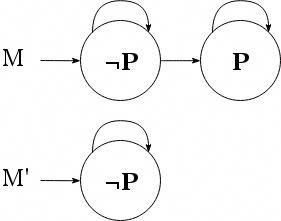
\includegraphics[width=\textwidth]{ltl-inexpressible.png}
            \end{minipage}

            CTL would express this as \(AG(EF\;\text{P})\): from any state, there's always a path to a state where P holds.
        }
        \subsubsection*{CTL can't, LTL can}
        {
            % pg 107
            % Finish this off quickly, do final lecture that I skipped, then supo work.
            % That's all the revision time I can spare for Hoare, chalk it up as done and move on to MSS?
            % Could do with skimming over Types and CompArch to refresh.
        }
    }
}
\end{document}